%%%%%%%%%%%%%%%%%%%%%%%%%%%%%%%%%%%%%%%%%
% University Assignment Title Page 
% LaTeX Template
% Version 1.0 (27/12/12)
%
% This template has been downloaded from:
% http://www.LaTeXTemplates.com
%
% Original author:
% WikiBooks (http://en.wikibooks.org/wiki/LaTeX/Title_Creation)
%
% License:
% CC BY-NC-SA 3.0 (http://creativecommons.org/licenses/by-nc-sa/3.0/)
%
%%%%%%%%%%%%%%%%%%%%%%%%%%%%%%%%%%%%%%%%%
%\title{Title page with logo}
%----------------------------------------------------------------------------------------
%	PACKAGES AND OTHER DOCUMENT CONFIGURATIONS
%----------------------------------------------------------------------------------------

\documentclass[12pt]{article}
\usepackage[english]{babel}
\usepackage[utf8x]{inputenc}
\usepackage{natbib}
\usepackage{amsmath}
\usepackage{listings}
\usepackage{color}
\usepackage{tabu}
\tabulinesep=1.2mm
\usepackage[explicit]{titlesec}
\usepackage{url}
\usepackage{subfig}
\usepackage{graphicx}
\usepackage{grffile}
\usepackage{mwe}
\usepackage[section]{placeins}

\usepackage{booktabs}
\usepackage{multirow}

\def\code#1{\texttt{#1}}

\begin{document}

\begin{titlepage}

\newcommand{\HRule}{\rule{\linewidth}{0.5mm}} % Defines a new command for the horizontal lines, change thickness here

\center % Center everything on the page
 
%----------------------------------------------------------------------------------------
%	HEADING SECTIONS
%----------------------------------------------------------------------------------------

\textsc{\LARGE University of St Andrews}\\[1.5cm] % Name of your university/college
\textsc{\Large CS4204 Coursework 1}\\[0.5cm] % Major heading such as course name
\textsc{\large }\\[0.5cm] % Minor heading such as course title

%----------------------------------------------------------------------------------------
%	TITLE SECTION
%----------------------------------------------------------------------------------------

\HRule \\[0.4cm]
{ \huge \bfseries Parallel Patterns}\\[0.4cm] % Title of your document
\HRule \\[1.5cm]
 
%----------------------------------------------------------------------------------------
%	AUTHOR SECTION
%----------------------------------------------------------------------------------------


\Large \emph{Author:}\\
 \textsc{150008022}\\[3cm] % Your name

%----------------------------------------------------------------------------------------
%	DATE SECTION
%----------------------------------------------------------------------------------------

{\large \today}\\[2cm] % Date, change the \today to a set date if you want to be precise

%----------------------------------------------------------------------------------------
%	LOGO SECTION
%---------------------------------------------------------------------------------------


\includegraphics[width = 3.1cm]{images/standrewslogo.png}
 
%----------------------------------------------------------------------------------------

\vfill % Fill the rest of the page with whitespace

\end{titlepage}

\section*{Goal}

To implement and evaluate a library for parallelising C programs, using PThreads, locks, and queues. 

\section{Blocking Queue}

The implementation of parallel task handlers would have to accumulate their outputs and buffer their inputs in a thread safe way, and so a blocking queue was necessary. \code{queue.h} provides an interface for a queue to be used by other components, and \code{queue.c} provides an implementation.

The queue is a linked list structure, where each node in the list has a reference to the element next in line. The queue structure tracks the last in line for adding new nodes, and the first in line for removing nodes. A conditional variable is used to notify threads waiting to add or remove elements that the size of the queue has changed, and a normal mutex is used to ensure that only one node is able to perform the addition or removal at a time (effectively creating a monitor). Figure \ref{fig:queue} shows a queue struct with a series of node structs.

\begin{figure}[!ht]
	\centering 
	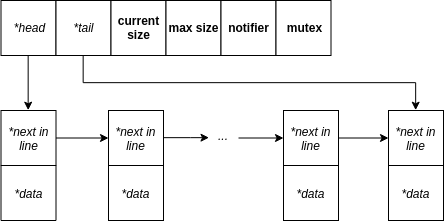
\includegraphics[width=0.8\linewidth]{images/queue}
	\caption{Queue structure, showing head and tail pointers, and each member of queue referencing the next.}
	\label{fig:queue}
\end{figure}

The blocking queue was tested for correctness by writing a simple test program that would create a queue, and spawn a large number of threads. Half of which would enqueue and the other dequeue elements and print what they did and when they were finished. If the queue was not thread safe, then threads would either block permanently due to the loss of elements in the list during insertion and removal, multiple threads would dequeue the same element, and elements could be left over despite an even number of inserts and removes. Whilst this is clearly not an exhaustive test, it was enough to provide confidence in the implementation. Use \code{make queuetest} then \code{./queuetest} to compile and run the tests. Figure \ref{fig:queuegrind} shows the output of \code{queuetest} when run using \code{valgrind --leak-check=full -v ./queuetest}.

\begin{figure}[!ht]
	\centering 
	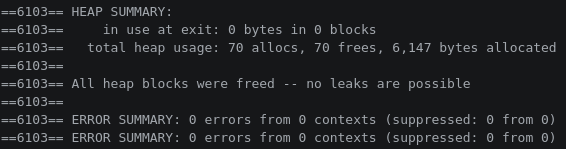
\includegraphics[width=\linewidth]{images/queuegrind}
	\caption{Valgrind output when running queue test.}
	\label{fig:queuegrind}
\end{figure}

\section{Steps}

The project was started with the intention of implementing nested parallel patterns. This required defining components that would be able to integrate both with pipelines and parallel farms. This component is referred to as a \code{Step}. Figure \ref{fig:step} shows visualises a step, with an input queue, a function to apply, and an output queue to place data once processed.

The step API is listed in \code{step.h}, and provides three methods: Step creation, destruction, and shutdown signalling. Step creation requires providing an input and output queue (that can't be the same queue), as well as the function to apply which could take any number of parameters and return anything. 

Originally, each step would spawn a single worker thread on creation which would run a function that would continuously poll the input queue for data to process. Upon receiving \code{NULL}, the worker thread terminates. The shutdown signal method adds NULL to the given steps input queue in order to trigger this shutdown. If multiple steps share an input queue then a NULL would have to be supplied for each consuming worker thread to ensure they all terminated correctly.

\begin{figure}[!ht]
	\centering 
	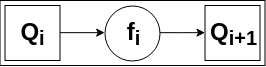
\includegraphics[width=0.45\linewidth]{images/step}
	\caption{Single step without input queue $Q_i$, output queue $Q_{i+1}$ and a function $f_i$.}
	\label{fig:step}
\end{figure}

\section{Filter}

Inspired by the Java 8 Streams API (and since it is a useful feature), I also wanted to include the ability for a step to filter data. An example of filters in pipelines is a graphics engine removing features that are out of view from the pipeline to avoid unecessary processing. 

Since NULL would terminate the worker thread for a step, I needed to differentiate between a filter function returning NULL (i.e. data was filtered) and the termination signal NULL. This was done by wrapping each instance of input data to the queues in a Task structure. A NULL task would be used as the termination signal. If a step was specified to be a filter, and its function outputted NULL, then the task would not be forwarded. This allowed NULL data to be passed through the pipeline also, and so developers using the library would not have to worry about their return data terminating the pipeline. Instead, they would return NULL from any function they wanted to act as a filter. 

\section{Ordering}

If inputs were to be processed in parallel, then there are many situations where ordering would have to be restored to the outputs. This was achieved by grouping inputs into \code{Batch}s, as shown in figure \ref{fig:batch}. When the user submits an array of data to be processed, an array of tasks are created for each data point in the order of the original data. Then the batch is created to track the number of tasks, the number that are completed, and the number that remain after filtering has occurred.

\begin{figure}[!ht]
	\centering 
	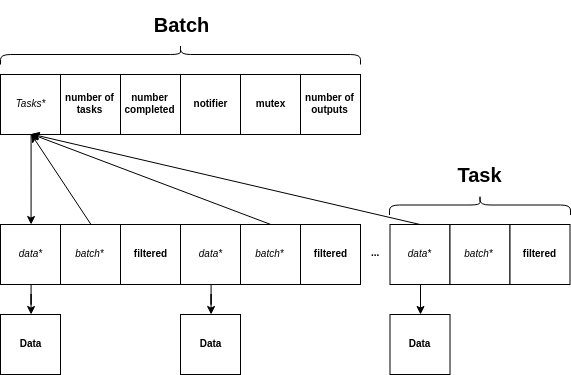
\includegraphics[width=0.8\linewidth]{images/batch}
	\caption{Structure of a task and batch.}
	\label{fig:batch}
\end{figure}

When a filter step receives a NULL output, it increments the batch counter by obtaining the batch lock and incrementing the completed count. Since tasks could be completed on multiple threads, this increment had to be performed in a thread safe manner.

Once satisifed with the single worker per step implementation, the ability to have multiple worker threads per step was then implemented. Figure \ref{fig:multiplestep} shows a step that has three worker threads each applying a function to inputs from the same queue and placing the return values in the same queue. This allowed steps to operate as simple parallel farms. It was noted that since each thread would share the same input queue, increasing the number of worker threads would increase the level of contention when trying to dequeue and enqueue tasks due to the blocking queues locking mechansim. 

\begin{figure}[!ht]
	\centering 
	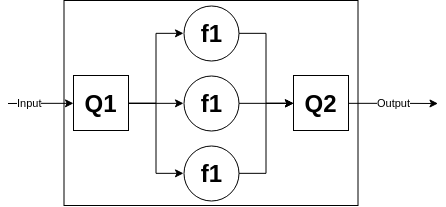
\includegraphics[width=0.8\linewidth]{images/farm}
	\caption{Step with multiple workers.}
	\label{fig:multiplestep}
\end{figure}

\begin{figure}[!ht]
	\centering 
	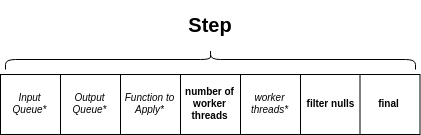
\includegraphics[width=0.8\linewidth]{images/stepstruc}
	\caption{Components of \code{struct Step}.}
	\label{fig:stepstruc}
\end{figure}


The step implementation and filter functionality was tested by iteratively building steps with a variable number of worker threads and a variable number of inputs and checking that the correct outputs were received. The normal step test would multiple each input by two, and the filter test would remove even numbers from the input. Use \code{make steptest} then \code{./steptest} to compile and run the test. The output from an example test run is shown in figure \ref{fig:steptest}. The tests were also run with valgrind to check that no memory leaks were occurring (figure \ref{fig:stepgrind}).

\begin{figure}[!ht]
	\centering 
	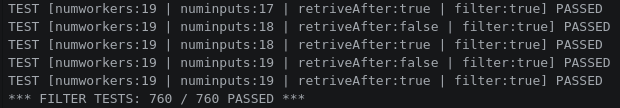
\includegraphics[width=\linewidth]{images/steptest}
	\caption{Output of filter step tests using combinations of 1 to 19 worker threads and 0 to 19 inputs, where output retrieval is performed before and after signalling the worker threads to terminate.}
	\label{fig:steptest}
\end{figure}

\begin{figure}[!ht]
	\centering 
	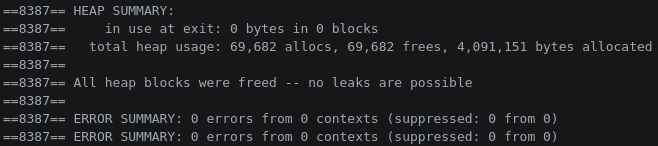
\includegraphics[width=\linewidth]{images/stepgrind}
	\caption{Valgrind output when running step test.}
	\label{fig:stepgrind}
\end{figure}

\section{Pipeline} 

The pipeline pattern is where a series of functions are applied to some input in a given order. Often the analogy of a conveyor belt is used, as inputs can flow continuously and functions can be applied simultaneously to inputs that are at different stages in the pipeline.

Figure \ref{fig:pipe} shows how a pipeline was implemented for this submission. An array of functions are submitted on creation of the pipeline, along with the number of worker threads that should run for each stage in the pipeline. The pipeline interface allows for inputs to be added to a queue, where they will wait to be processed, and for outputs to be polled from the outgoing queue. 

\begin{figure}[!ht]
	\centering 
	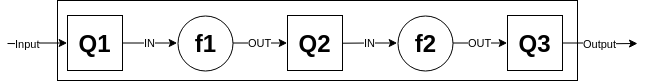
\includegraphics[width=\linewidth]{images/pipe}
	\caption{Pipeline abstraction, where Q signifies a blocking queue, and f signifigies a function being applied.}
	\label{fig:pipe}
\end{figure}

The pipeline was defined to consist of a series of steps. The thread for step $i$ would poll queue $Q_i$ for an input $x$ to process, compute $f(x)$, then add the output to queue $Q_{i+1}$. $Q_0$ and $Q_{n+1}$ are the input and output queues made accessible by the pipeline interface, where $n$ is the number of functions in the pipeline. The number of queues needed can be calculated using the number of functions $n+1$. 

One of the difficult design decisions was setting how to manage the size of the queues that would buffer data between each step in the pipeline. Figure \ref{fig:qsize} shows three situations: equal producers and consumers, more producers thatn consumers, and more consumers than producers. The relative speed of the producers and consumers would also have to be considered (e.g. how quickly the producer produces). The processing time of the pipeline would be dependent on the speed of the slowest step if queues are assumed to always have data to consume at each step (i.e. no waiting).

\cite{buffer} describe and try to tackle the problem of choosing these buffer sizes. They conclude that in a homogeneous pipeline (where each step takes the same time), equal buffer sizes at each step is efficient. They also provide optimised buffer size allocations for pipelines where each step takes incrementally longer, for example. 

I opted for the size of the input queue at each step to be equal to the number of consumer threads at the next step. This would at least ensure that as long as the producer equalled or outpaced the consumer, the the consumer would never have to wait for data to process. This could be wasteful in terms of memory however if the producer is unable to fill the queue due to the consumer being quicker.

\begin{figure}[!ht]
	\centering 
	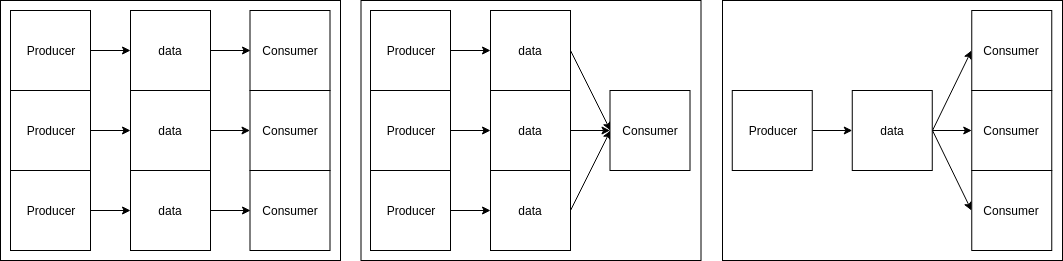
\includegraphics[width=\linewidth]{images/qsize}
	\caption{Scenarios when creating queues.}
	\label{fig:qsize}
\end{figure}

\begin{figure}[!ht]
	\centering 
	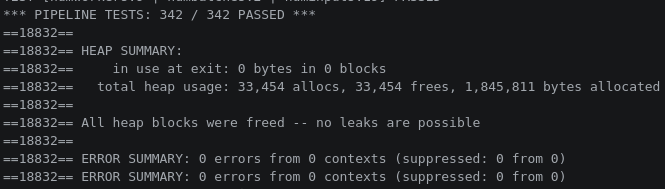
\includegraphics[width=0.8\linewidth]{images/pipetest}
	\caption{Output of valgrind when running \code{pipetest}.}
	\label{fig:pipetest}
\end{figure}

\section{Parallel Farm}

The parallel farm pattern involves a pool of worker threads that remain idle until assigned a task by a coordinator. Once a worker thread completes its task, it then returns to being idle until a new task is assigned. Parallel farms are useful as they avoid the overhead involved in creating threads. 

As mentioned earlier, \code{Step}s already provided a method of having multiple worker threads processing from the same input queue, and the pipeline API already contained a way of constructing steps and submitting tasks. Therefore the farm API simply wrapped a pipeline instance with a single step and multiple worker threads.

\section{Evaluation}

The provided convolution program was going to be used for evaluation as it was clearly appropriate to use a pipeline when processing the images iteratively. Unfortunately I was unable to get the C library to compile with \code{gpp}.

Instead, computation was simulated by varying sleep times for each function. Three phases of the geometry phase in a graphics pipeline were used in order to test the effectiveness of the implementation and compare it to a serial computation: clipping, transformation, and rasterisation. The first step removes object outside of the visual volume from being processed later, the second involves scaling the content to the given viewport, and the last produces pixel information for each point in the resulting image. 

Transformation was assumed to take the shortest time since it is a simple vector multiplication, clipping the next longest, then finally rasterisation taking the longest. The processing time ratio adopted was 2:1:3. Each task was assumed to be able to be parallelised. 

The first evaluation test is based on the experiments in \cite{grppi} which used different pipeline compositions as shown in figure \ref{fig:grppi}. GRPPI was also used as an inspiration for the API design of this submission, so it seemed appropriate to evaulate it using a similiar experiment. Three stages were used, which would each either have 1 or 3 worker threads, written as \code{p} if 1 and \code{f} if 3. Using the ratio discussed earlier, the relative processing delays were scaled up by factors of 10 from $1ns$ to $10000000ns$. The configurations are summarised in table \ref{tbl:exp1}. For each configuration in each row of the table, the computation was also performed single threaded for comparison. The initialisation and teardown times were included in the pipeline execution times, which was expected to result in a cutoff point where the multithreaded pipeline became more efficient.

\begin{figure}[!ht]
	\centering 
	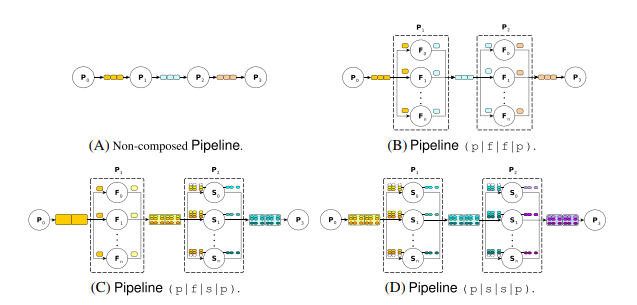
\includegraphics[width=\linewidth]{images/grppi}
	\caption{Composed pipeline structures from \cite{grppi}.}
	\label{fig:grppi}
\end{figure}


\begin{table}[]
\centering
\resizebox{\textwidth}{!}{%
\begin{tabular}{@{}ccc|lll|l@{}}
\toprule
\multicolumn{3}{c|}{\textbf{Steps}}                 & \multicolumn{3}{c|}{\textbf{Delay (ns)}}                                                                         & \multicolumn{1}{c}{\multirow{2}{*}{Number of Inputs per Batch}} \\
\textit{Step 1} & \textit{Step 2} & \textit{Step 3} & \multicolumn{1}{c}{\textit{Step 1}} & \multicolumn{1}{c}{\textit{Step 2}} & \multicolumn{1}{c|}{\textit{Step 3}} & \multicolumn{1}{c}{}                                            \\ \midrule
P               & P               & P               & 2,20,...2000                        & 1,10,...1000                        & 3,30, ... 3000                       & 1, 10, 100                                                      \\
P               & P               & F               & 2,20,...2000                        & 1,10,...1000                        & 3,30, ... 3000                       & 1, 10, 100                                                      \\
P               & F               & P               & 2,20,...2000                        & 1,10,...1000                        & 3,30, ... 3000                       & 1, 10, 100                                                      \\
P               & F               & F               & 2,20,...2000                        & 1,10,...1000                        & 3,30, ... 3000                       & 1, 10, 100                                                      \\
F               & P               & P               & 2,20,...2000                        & 1,10,...1000                        & 3,30, ... 3000                       & 1, 10, 100                                                      \\
F               & P               & F               & 2,20,...2000                        & 1,10,...1000                        & 3,30, ... 3000                       & 1, 10, 100                                                      \\
F               & F               & P               & 2,20,...2000                        & 1,10,...1000                        & 3,30, ... 3000                       & 1, 10, 100                                                      \\
F               & F               & F               & 2,20,...2000                        & 1,10,...1000                        & 3,30, ... 3000                       & 1, 10, 100                                                      \\ \bottomrule
\end{tabular}%
}
\caption{Configurations for experiment.}
\label{tbl:exp1}
\end{table}





\section*{Conclusion}

\bibliographystyle{unsrt}
\bibliography{mybib}

\end{document}
